\section{Experiments}
\label{experiments}

\begin{figure}
    \centering
    \subfigure{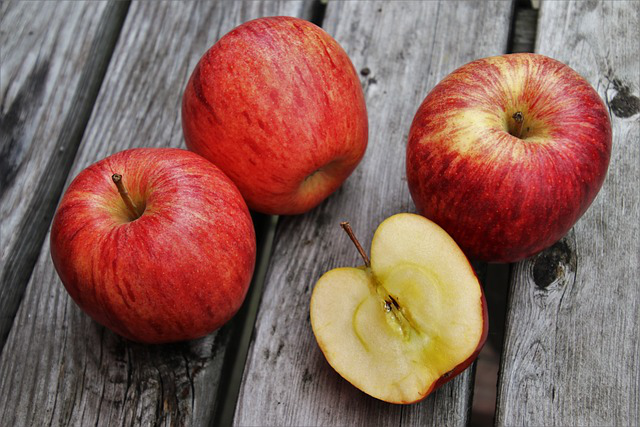
\includegraphics[width=0.24\textwidth]{apples.png}}
    \subfigure{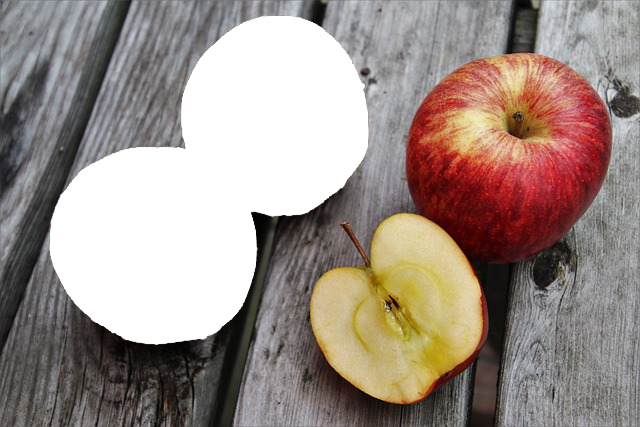
\includegraphics[width=0.24\textwidth]{apples_fore.png}}
    \subfigure{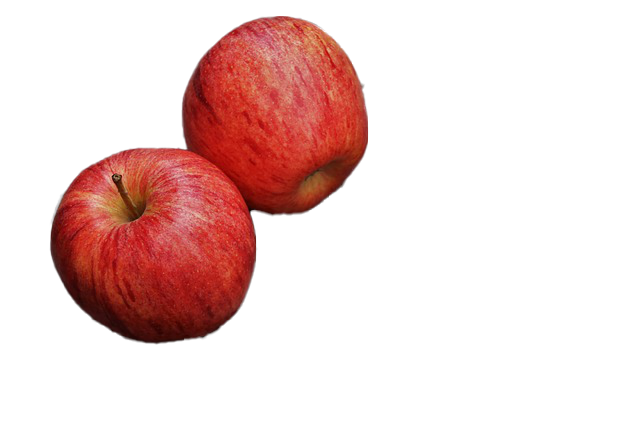
\includegraphics[width=0.24\textwidth]{apples_back.png}} \\
    \subfigure{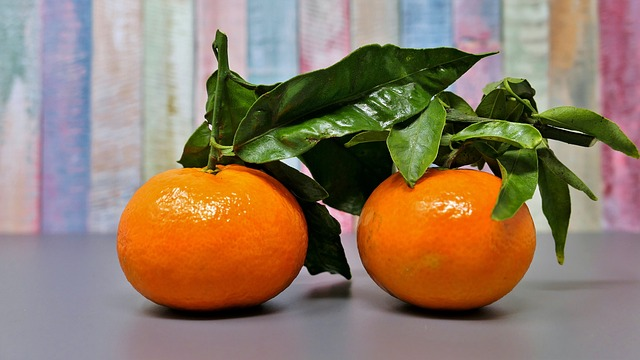
\includegraphics[width=0.24\textwidth]{mandarins.png}}
    \subfigure{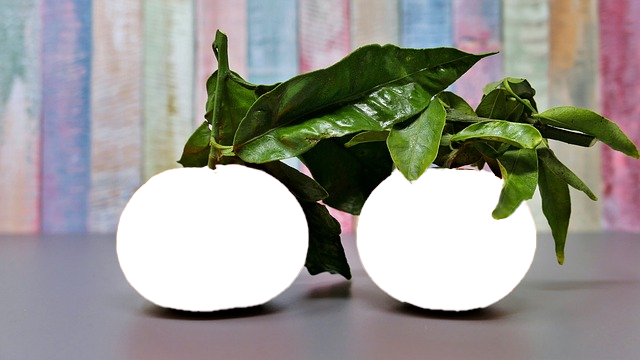
\includegraphics[width=0.24\textwidth]{mandarins_fore.png}}
    \subfigure{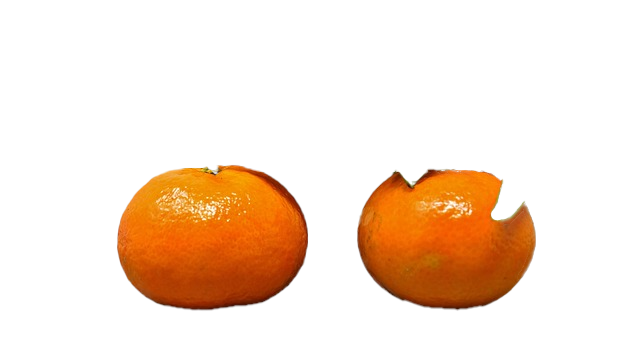
\includegraphics[width=0.24\textwidth]{mandarins_back.png}}
    \caption{Training datasets with foreground and background scribbles}
    \label{data}
\end{figure}

\begin{table}
    \centering
    \caption{Performance evaluation on the "Mandarins" dataset}
    \begin{tabular}{lll}
        \toprule
              & \multicolumn{2}{c}{IoU}                \\
        \cmidrule(r){2-3}
        Model & No Teacher              & With Teacher \\
        \midrule
        FICNN & 0.9152                  & 0.9345       \\
        Our   & 0.9422                  & 0.9592       \\
        \bottomrule
    \end{tabular}
    \label{exp}
\end{table}

\begin{figure}
    \centering
    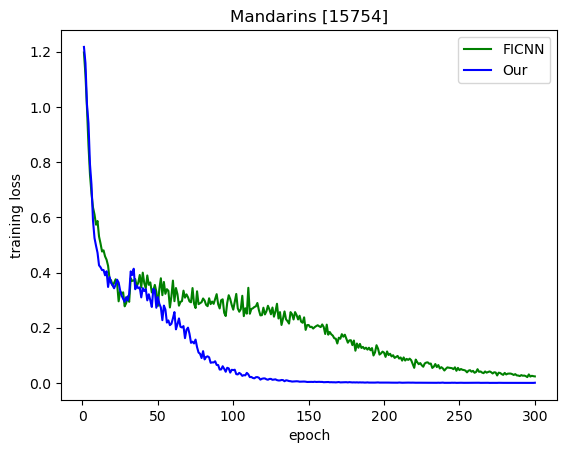
\includegraphics[width=0.65\textwidth]{training.png}
    \caption{Training loss on the "Mandarins" dataset.
        The spike at epoch 30 is explained by the change of the loss function.}
    \label{training}
\end{figure}

\begin{figure}
    \centering
    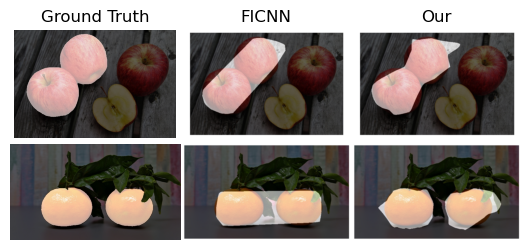
\includegraphics[width=0.65\textwidth]{resources/segmentation_result.png}
    \caption{Visual comparison of FICNN and our approach}
    \label{visual}
\end{figure}

In this study, we evaluated the performance of the proposed approach based on two datasets
extracted from scribbles presented on the Figure~\ref{data}.
The datasets "Apples" and "Mandarins" contain 3720 and 15774 labeled datapoints, respectively.

We compared our approach against a 3-layer FICNN (\cite{amos2017input}) with and without
a teacher network. The purpose of the teacher network is to provide both our composite network and FICNN
with the labels for the unlabeled pixels, since. The network can be arbitrarily complex or even omitted.

In the setting of scribble-based image segmentation, the amount of labeled pixels is usually low,
relatively to the size of the segmented image.
Therefore, as highlighted in the Table~\ref{exp}, the use of even a simple teacher
network leads to an increase in the quality of the resulting segmentation mask
without affecting the connectedness.
In our experiments, we employed a fully-connected network
with two hidden layers of 130 neurons each.

The training was performed jointly. In the Section~\ref{loss} we explain how the
loss function used for training is constructed.
We used Adam optimizer with a static learining rate of $10^{-4}$.
Each configuration was trained for 300 epochs with the batch size of 1500.
In each epoch, 1200 random datapoints from the dataset are combined with the input
in order to increase generalization abilities of the model by making it less prone to overfitting.

Our experiments show that our approach allows to achieve higher segmentation quality
as compared to the FICNN.
Moreover, due to the fact that our model performs segmentation only based
on the positional information of each pixel in the dataset, it is completely invariant to noise.

The Figure~\ref{visual} provides visual comparison of our model against FICNN.
We can see that our approach allows more flexibility.
However, further investigation is needed to determine the reason of having two path-connected
regions in the segmentation mask of the Mandarins dataset.
Our conjecture is that the model learns to preserve the connectedness
in the latent space despite the segmented objects being disconnected in the data space.

We can also see on the Figure \ref{training}, that our model converges faster than FICNN.

\subsection{Loss function}
\label{loss}

In order to perform joint training of both our model and the teacher network,
we introduce a loss function which evolves during the training process.
The base loss function is binary cross-enrtopy loss:

\[
    L(y_{t}, y, \hat{y}) = BCE(y_{t}, \hat{y}) + BCE(y, \hat{y})
\]

where $y_{t}$ and $y$ are the predictions of the teacher network and our model, respectively,
and $\hat{y}$ is the ground truth.

After 30 epochs, we add the mean squared error between the predictions of our model
and the rounded predictions of the teacher network.
Thus, the loss function evolves to the following form:

\[
    L(y_{t}, y, \hat{y}) = BCE(y_{t}, \hat{y}) + BCE(y, \hat{y}) + MSE(y, round(y_t))
\]

After 200 epochs, we require our model to match the predictions of the teacher model more by
omitting the rounding of its predictions and using $y_t$ unmodified.